In this project, the goal is to label all faces in the given image as mask/no mask

We'll need to determine which of these women is wearing a medical mask.

\begin{figure}[H]
    \centering
    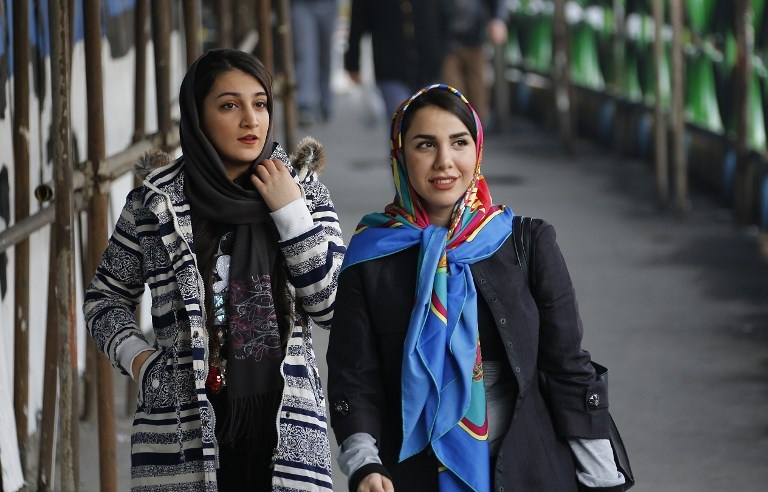
\includegraphics[width=0.7\textwidth]{Orig.jpeg}
    \caption{Original Image}
    \label{fig:Orig}
\end{figure}


\begin{figure}[H]
    \centering
    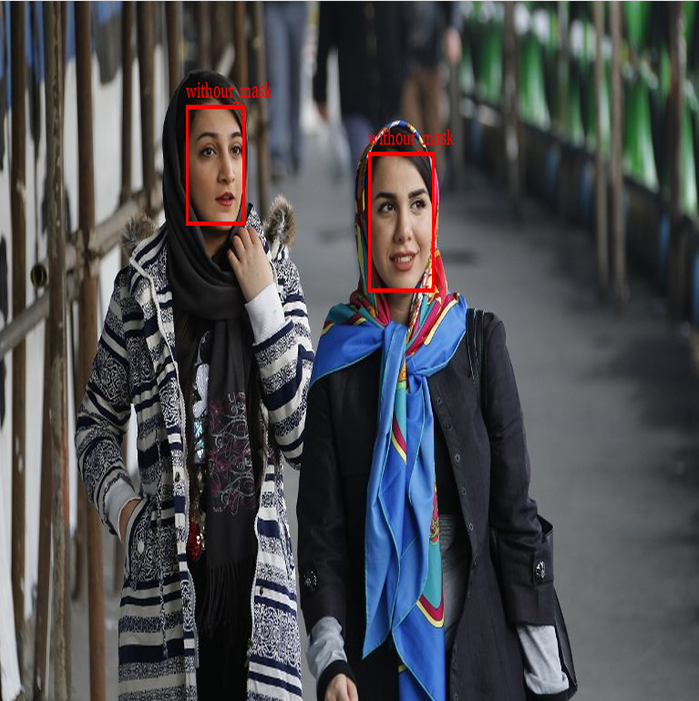
\includegraphics[width=0.7\textwidth]{twoImage-Annotated.png}
    \caption{Annotated Image}
    \label{fig:Annotated}
\end{figure}

\subsection{Expected Achievements}
Contents:
\begin{enumerate}
  \item Take both datasets and use augmentation to improve pictures.
  \item Pick two models best suits (CNN) our problem \& search for the best hyper parameters.
  \item Train two models on my datasets and save it for later use.
  \item Test it using a GUI or a great integration script, and run on an unseen test images
\end{enumerate}
